\chapter{Time-Oriented Visual Exploration}\label{chap:basics}

%%%%% Problems %%%%%%%%%%%%%
This chapter identifies the factors involved in the visualization process of time-oriented data. By following a problem-oriented approach section \ref{problems} sketches the problems that appear if the analyzed data has a high data volume. In particular limited monitor resolution is described. Section \ref{data} addresses the data and section \ref{tasks} the user tasks. In section \ref{vis} time-oriented visualizations are selected.

 \section{Understanding the Problem}\label{problems}
The current challenge in \gls{BIV}  is how to handle large amounts of data and to display them in an effective manner. Yet, large amounts of data causes conflicts with effective data representation. One conflict is visual clutter as shown in figure \ref{fig:first}. Visual clutter denotes overlapping and distracting data items. Clutter is caused by similar data items which overlap. If similar yet not identical data items are visualized at once, items cannot be distinguished anymore as in figure \ref{fig:second}. 
 
\begin{figure}
 \centering
\subfloat[Parallel Coordinates with Cluster.]{\label{fig:first}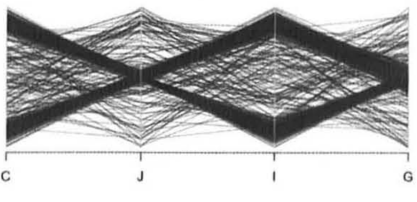
\includegraphics[width = 0.46\textwidth]{src/images/PC1}}
\qquad
\subfloat[Parallel Coordinates without  Cluster.]{\label{fig:second}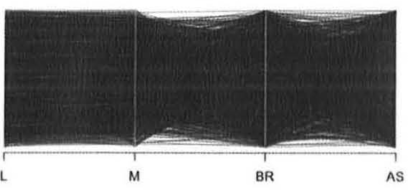
\includegraphics[width = 0.46\textwidth]{src/images/PC2}}
\caption[Parallel Coordinates]{From \cite{Tatu2010}.}
\end{figure}
 
 Visual clutter arises if the entire data set necessary to provide the user with an overview is displayed. Displaying an overview is a basic yet important task because it navigates the user through the data and allows for further analysis. Thus, the problems of large data can be summarized as follows: 
\par
\textit{Overlap}: 
The visualization of large data causes overlap. Depending on the drawing order the picture may look different and cause different interpretations even though the underlying data is the same. Visualization techniques need to avoid visual overlap (\ref{vis}, \ref{multi-resolution}). 
\\*
\textit{Visual Noise}: 
Even if data items are not overlapping, data in large data sets might be too similar to one another. Thus, the user cannot differentiate distinct items on the screen. A solution is discussed in \ref{aggregationmarkers}.
\\*
\textit{Limited monitor resolution}:
Even if large monitors are used to visualize data, in the end the available pixels on the monitor are smaller than the number of data items in a data set. This problem will be discussed in \ref{resolution}.
\\*
\textit{Limited visual perception}:
Moreover, human perception is limited in the number of patterns and pixels which will be reviewed in \ref{perception}.
\\*
\textit{Finding regions of interest}:
If the data set is too large and overlap occurs, the user faces the challenge of finding an interesting subset in the data. Thus, appropriate interaction techniques are necessary (\ref{search}).
\\*
\textit{Navigation}:
To find a region of interest the user might zoom in. But then another challenge occurs in navigating in the large data set. As there are too many data points the user might loose the overview and get lost in data analysis. Navigation techniques are methods to overcome this problem (\ref{navigation}).
\\*
% \textit{Information Loss}:
% While reducing the number of data items to present them on the limited screen information in the data can be lost. The important question is which data characteristics to keep such that the user tasks can still be supported.
\par
To propose a solution to the problems of large-scale data visualization it is important to gain understanding of the process of visualization, which is described in the Visualization Pipeline in figure\ref{fig:vispipeline}. 
\begin{figure}[H]
    \centering
        \scalebox{.5}{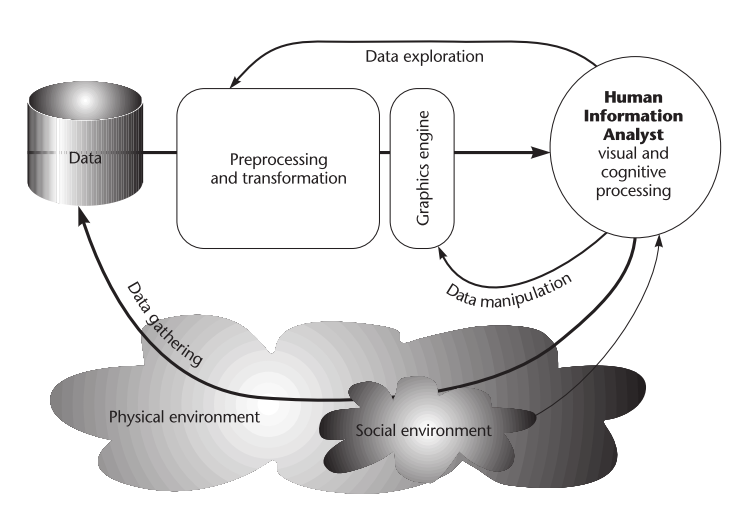
\includegraphics{src/images/VisPipeline}}
    \caption[Visualization Pipeline]{Visualization Pipeline}
    \label{fig:vispipeline}
\end{figure}

As the visualization pipeline shows, the process of visual analysis is influenced by three entities: the data, the user and the visualization.
The three entities can also be described as \textit{domains}: data-domain, user-domain and visualization-domain. The data-domain represents \textit{what} is visualized. The user-domain explains \textit{why} the problem is visualized and the visualization-domain characterizes \textit{how} the problem is visualized. Thus, we will explore the three domains in the following sections to answer the following questions: 

\begin{itemize}
    \item The User Domain: Why is it presented?
    \item The Data Domain: What is presented?
    \item The Visualization Domain: How is it presented?
\end{itemize}

Given the data as input, visual clutter can be reduced by adapting the steps \textit{preprocessing \& transformation}, \textit{graphics engine}, \textit{visualization} and \textit{data manipulation}. Preprocessing involves data preparation such as database joins or data cleansing. The graphics engine covers rendering processes and data formats. This part will not be covered in this work as it is out of scope since the focus of this work is on visualization techniques. The visualization step considers visualization techniques. Data manipulation describes interaction techniques.  

% User Tasks
\section{The User Domain} \label{user}
In the visualization pipeline the user has the role of the data analyst, which is why every visualization tool should consider the user perspective with its general human perception and the time-oriented user tasks.
\par
\subsection{Visual data exploration}
Humans use visualizations to see what they are thinking of. Hereby, visualizations make use of 
the most elaborate human sense - the visual sense. By presenting data in a visual manner information visualization reduces the cognitive overload. It makes abstract relationships concrete. 

Business visualization is used in the process of \textit{problem-solving}. In order to confirm or to build hypotheses the user visualizes data to gain insights and to interact with the data. Thereby, visualization enhances the required working memory for solving problems\cite{Card1999}. Visualizations support the user in perceiving patterns and making problems obvious. Thus, visualizations support the business user in problem-solving. For time-oriented data the user has specific goals in mind which are the so-called user tasks (\ref{tasks}). Especially, pattern-related tasks are supported by visual data exploration. Visualizations can present large data sets. Yet, perceptual limitations determine the presentation of massive amounts of data.

\subsection{Perceptual limitations} \label{perception}
% What can humans perceive? How many pixels? 
The brain is limited to perceiving pixels on the screen as well as patterns created by visualizations. Since space in the brain is represented differently from the screen, the term computer monitor pixels requires a brain equivalent for screen pixels. We call them brain pixels. According to  \cite{Ware2012} brain pixels are nearly represented by ganglion cells. Ganglion cells are neurons which send information to the cortex. In the fovea one ganglion cell cares about one single cone. In the periphery one ganglion cell handles thousand of rods and cones. Thus, the brain pixel resolution in the fovea is much higher than in the periphery. The brain aggregates pixels and adheres to multiple resolution which is also used in visualization known as multi-resolution.
To model how many data items are perceived by the human brain it is important to make the following distinction: 
\\*
\textit{\gls{TBP} = total amount of brain pixels which is stimulated by the screen pixels}\\*
and unique stimulated brain pixels: \textit{\gls{USBP} = \gls{TBP} - redundant brain pixels}.\\*
\gls{USBP} are the number of pixel who determines the human perception of data items. A measure of display efficiency (\gls{DE}) is the ratio of \gls{USBP} and screen pixels (\gls{SP}): \textit{\gls{DE} = \gls{USBP}/ \gls{SP}}.

Figure \ref{fig:DE} shows that a monitor larger than 40cm wide does not increase the display efficiency any further. For large data sets this allows for the conclusion that the perception of large data has a limit in the human perception. The current average monitor size (which approximately is  40-50cm) is sufficient to respond to the number of \gls{USBP}.

\begin{figure}[H]
    \centering
    \scalebox{.3}{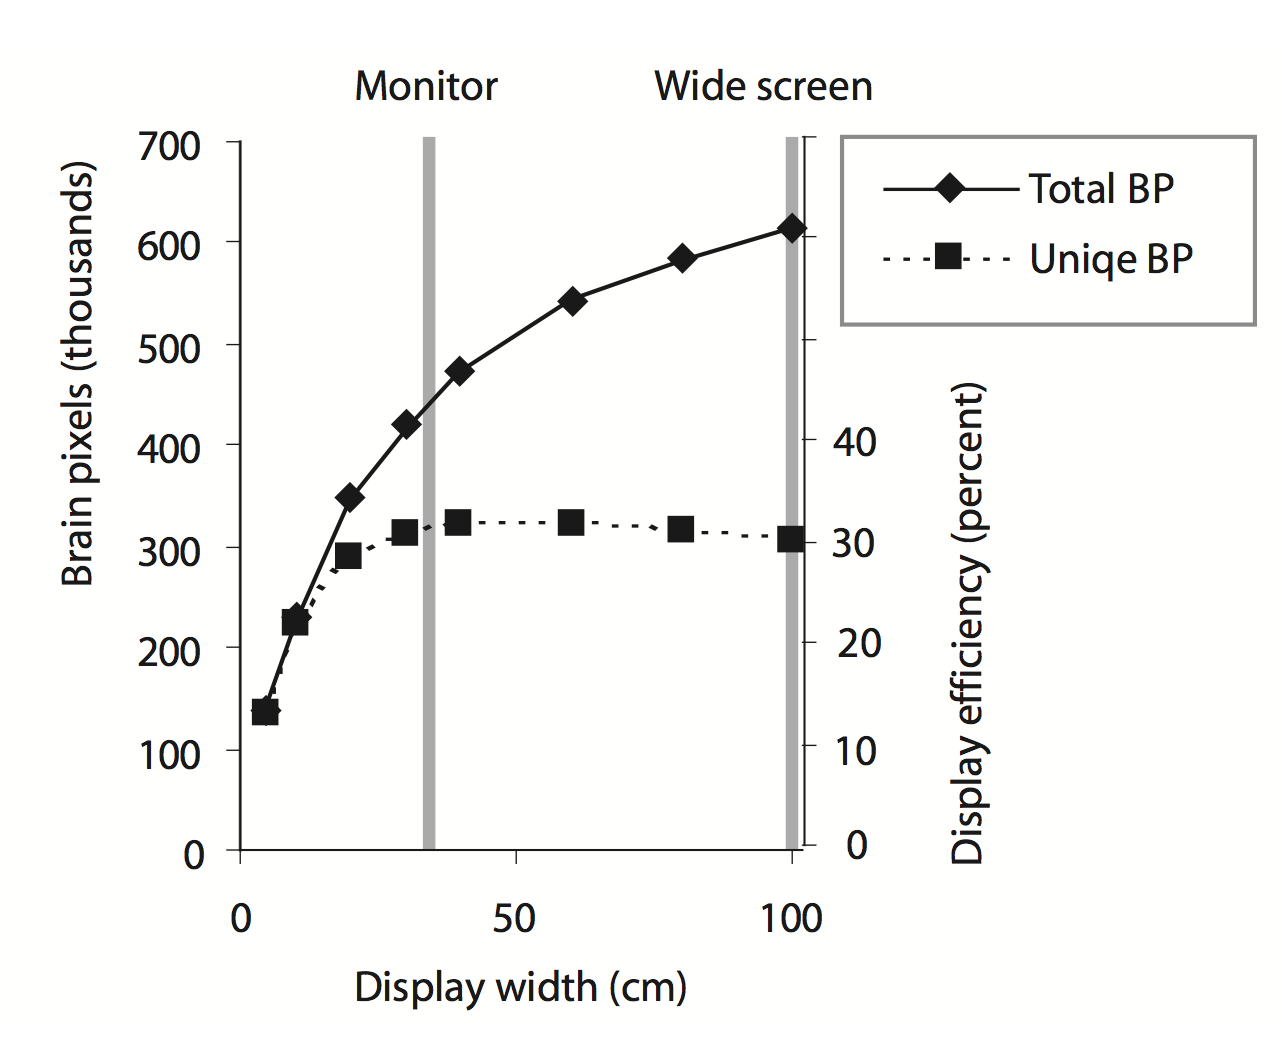
\includegraphics{src/images/DE}}
    \caption[Display Efficiency]{Simulation of display efficiency by exposing the brain to a one million pixel screen. From  \cite{Ware2012}.}
    \label{fig:DE}
\end{figure}

The human visual system is able to perceive 15mio pixels per eye  \cite{Deering1998}. Assuming that the amount of perceivable pixels for two eyes is larger than 15mio pixels but smaller than 30mio pixels due to the overlap of the field of view, the maximum amount of perceivable pixels (\gls{PP}) is:
\begin{math}
15 mio. \leq pp < 30 mio.
\end{math}

Nevertheless, the important question is not the amount of \gls{PP} but whether the data structure, patterns, trends and further information in the data can be perceived - the human brain is after all, a pattern detection machine  \cite{Ware2012}. If we consider the brain's ability to detect patterns, aggregation methods for visualizations are not only tolerated but moreover recommended. Moreover, the main concern for visualization techniques should be the perception of patterns: trend, outliers, clusters. \label{pattern}
\par

\subsection{Time-oriented user tasks} \label{tasks}
The business user is a person that is interested in verifying existing hypotheses (verification) and discover new patterns (discovery). By using the visualization tool he expects it to assist him in analyzing the data, finding critical issues and automatically performing analysis \cite{Brachman1996}. Verification and discovery in the analysis of time-oriented data can be split in seven major tasks  \cite{Esling2012}.\\*

\textbf{T1: Query by Content}
\\*
Given a known query, \textit{query by content} describes the retrieval of similar items to this query. In time-oriented data, query by content returns the \textit{k} most similar time series to the queried time series.
\\*
\textbf{T2: Clustering}\\*
Clustering is the process of finding expressive groups (clusters) in the data. Therefore, the data set is divided into subgroups according to some similarity measure. In the context of large time-oriented data, clustering is important to compare similar time-series.
\\*
\textbf{T3: Classification}\\*
In classification, the task is to find the right group the item belongs to. According to Aigner et al. temporal classification describes the preprocessing of finding the correct group for the given data or data set \cite{Aigner2008}. This task is important for large data in order to abstract the data and make it manageable. As this task is preprocessing and not data presentation or exploration we will not check whether the tools support the user in this task. 
\\*
\textbf{T4: Segmentation}\\*
Segmentation splits a time series into \textit{k} meaningful subsequences (segments)  \cite{Batyrshin2007}. 
\\*
\textbf{T5: Prediction}\\*
In Prediction, \textit{k} future events are predicted based on the past \textit{n} time series. This process is also known as \textit{forecasting}. 
\\*
\textbf{T6: Anomaly Detection} \\*
Anomaly detection points out events which behave in a different way than expected.
\\*
\textbf{T7: Pattern Discovery}\\*
Pattern discovery finds regularly appearing structures in a time series.  It covers the exploration of trends, outliers and clusters. Particularly in business, this is one of the most important tasks.
\par
The user tasks are the guideline in the research of large data visualization. If the user can successfully achieve his tasks with large data sets, the proposed criteria (\ref{success}) are successful.


% Data types for Information Visualization
\section{The Data Domain} \label{data}

With respect to large time-oriented data for business, we will consider three given characteristics of data: characteristics of business data, time-dependency and its size. Business data is collected in many different areas. Table \ref{table:applications} gives an overview of the applications: 

\begin{table}[H]
	\centering
	\caption[Business Applications]{Business Applications  \cite{Brachman1996,Tegarden1999}}
	\label{businessapplications}
	\begin{tabular}{ll}
	\toprule
	Marketing & Financial Sector \\
	Fraud Detection & Manufacturing and Production \\
	Operations Planning & Market Analysis \\
	Health Care & Network Management\\
	\bottomrule
	\label{table:applications}
	\end{tabular}
\end{table}
For each application area a number of publications covering different aspects exist. The analysis of every single application would go beyond our scope so we decided to consider data with the following characteristics only: 
\begin{enumerate}
    \item Data that is structured. 
    \item Data that is abstract.
    \item Data that is multivariate.
    \item Data that is discrete.
\end{enumerate}

\textbf{Structured data}: Data can come in many different forms. Unstructured data appears in text, speech and language processing. Structured data comes in tables in which each attribute is represented by one column and each row is one data item. The attributes can be either numerical or text-based. As business data is usually represented in tables  \cite{Borgo2013} we assume that business data is structured.\\*
\textbf{Abstract and Multivariate data}: The assumption of abstract and multivariate data is based on Tegarden's work in which he described business data as abstract, multivariate and discrete \cite{Tegarden1999}. 
\\*
\textbf{Discrete and time-oriented data}: A time-oriented data set contains data items which change over time. Each data item has a timestamp which is saved in one table-column. The time-dependency of the data structures the data by a given order. Every data item is mapped to a specific point in time with a smallest possible unit such as seconds. Time with a smallest unit is mapped to integer  \cite{Aigner2011} and thus we assume that time-oriented business data is discrete and has a given order.  \\*



\section{The Visualization Domain} 
\label{resolution}
Visualizations are usually mapped to a computer screen. In proposing solutions for limited monitor resolution one could propose larger displays. The Browser Display Statistics showed that the most popular display width is around 50 cm even though large wall-sized screens have been developed \cite{W3schools2017}. Sometimes, -depending on the department- two or three monitors are combined for a larger wall. Thus, the maximum number of pixels which can be used at the workspace ranges from monitors range from 786.432 pixels (1024x768) to 6.912.000 pixels(three monitors à 1920x1200). Large data sets fit into the screen but huge data exceed the maximal number of screen pixels. However, the discussion of human perception showed that larger monitors do not solve the problem of large data visualization. Instead, the important question is whether patterns are perceivable.
\par
\label{vis}
Usually time series data is visualized with line charts. However, line charts can only show \textit{univariate} data. Our selection of visualization techniques is based on Aigner et al.  \cite{Aigner2011} which presents current approaches to visualize time-oriented data. In this regard we focus on 34 techniques that can be used to show abstract, multivariate and discrete data (compare section \ref{data}). 
As the work of Aigner was published in 2011 we completed the set of techniques with current approaches based on the \href{http://survey.timeviz.net/}{TimeVizBrowser} a web-based collection of time-oriented techniques. Moreover, we consider only stand-alone visualization techniques - no systems, tools or software. In literature, a significant amount of publications describe new tools or systems which tackle the visualization of time-oriented data \cite{Hochheiser2004,Buono2005}. These tools usually are specific tools which can only be applied in a limited field. As we write this work with the perspective of business users, tools have to be generic and single-task systems are not appropriate.


We are aware that this discussion cannot be exhaustive as time-oriented data is a current research area and new visualization techniques are developed in rapid fashion.
Moreover, time-oriented data appears in different areas of business: E-commerce, Smart Health, E-Government, Science \& Technology, Security \& Public safety. Each sector collects different types of data and uses different applications, which makes it impossible to name every single existing visualization technique.


However, this work follows Keim's taxonomy of visualization techniques for large data. Their definition is explained in section \ref{related:class}.
